\section{Kết quả kiểm thử từng thành phần}
\label{sec:component_testing}

Trước khi tiến hành phân tích hiệu năng, các thử nghiệm chức năng được thực hiện để xác nhận rằng từng thành phần của hệ thống hoạt động đúng như thiết kế.  
Các log tiêu biểu và hình ảnh minh họa dưới đây cho thấy quá trình khởi tạo, kết nối, truyền dữ liệu định kỳ, phát hiện té ngã, xử lý cảnh báo và truyền hình ảnh.

\subsection{Module cảm biến đeo}
Module Quectel EC800K là thành phần thuộc module cảm biến đeo được kiểm tra để xác nhận khả năng giao tiếp AT command, thiết lập kết nối 4G và thu nhận dữ liệu GPS.  

Các bước kiểm thử bao gồm: khởi tạo UART, kiểm tra thông tin modem và SIM, đánh giá chất lượng sóng, cấu hình APN, kích hoạt PDP context, bật GPS và truy vấn tọa độ, sau đó tắt GPS và ngắt kết nối dữ liệu để tiết kiệm năng lượng.  

Kết quả cho thấy mô-đun hoạt động ổn định: thiết bị nhận diện đúng (EC800K), SIM sẵn sàng, tín hiệu mạnh (\texttt{+CSQ: 31,99}), kết nối dữ liệu thành công và thu được tọa độ GPS hợp lệ.

\textbf{Log tiêu biểu:}
\begin{minted}[fontsize=\footnotesize,breaklines]{text}
I (2329) SIM_4G: Received: Quectel EG800K
OK
I (5329) SIM_4G: Received: +CSQ: 31,99
OK
I (28339) SIM_4G: Received: +QIACT: 1,1,1,"9.204.251.200"
OK
I (34349) SIM_4G: Received: +QGPSLOC: 10.88862,106.77975
OK
\end{minted}

\textit{Kết luận:} Mô-đun 4G/GPS đã hoạt động đúng chức năng, đảm bảo hệ thống có thể gửi cảnh báo và thông tin định vị qua SMS/MQTT.

\subsection{Khởi tạo hệ thống và kết nối mạng}
Quá trình khởi tạo xác nhận rằng các mô-đun SIM4G-GPS, Wi-Fi và các tác vụ chính đều hoạt động bình thường, đảm bảo thiết bị sẵn sàng tham gia vào quá trình truyền thông và giám sát.

\begin{minted}[fontsize=\footnotesize,breaklines]{text}
I (9961) SIM4G_AT: Initializing SIM4G AT driver...
I (9981) SIM4G_AT: Successfully set APN to v-internet
I (10011) APP_MAIN: System initialization complete.
I (10021) APP_MAIN: Application started successfully
\end{minted}

\textit{Kết luận:} Hệ thống đã khởi tạo thành công, chứng minh nền tảng phần mềm và phần cứng được tích hợp ổn định.

\subsection{Kết nối MQTT và truyền dữ liệu}
Thiết bị ESP32 kết nối thành công với broker MQTT và thực hiện gửi bản tin định kỳ chứa thông tin định danh, trạng thái té ngã và dữ liệu GPS.  

\begin{minted}[fontsize=\footnotesize,breaklines]{text}
I (19961) USER_MQTT: MQTT_EVENT_CONNECTED
I (39991) JSON_WRAPPER: Created status payload:
{"device_id":"ESP32_DEV_76E48B","fall_detected":false,
 "latitude":0,"longitude":0,"has_gps_fix":false}
\end{minted}

\begin{figure}[H]
    \centering
    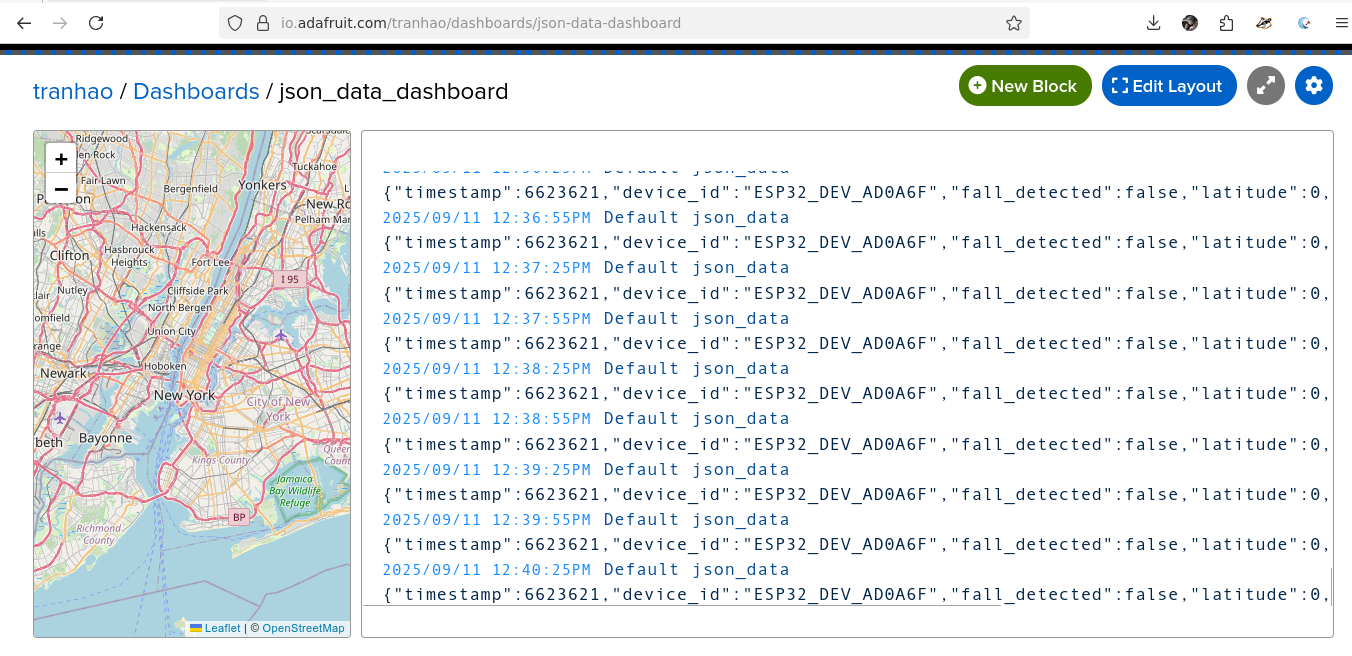
\includegraphics[width=0.8\textwidth]{figures/json_data_dashboard.png}
    \caption{Dashboard hiển thị bản tin MQTT từ thiết bị ESP32.}
    \label{fig:mqtt_dashboard}
\end{figure}

\textit{Kết luận:} Kết nối MQTT ổn định, đảm bảo thiết bị có thể truyền dữ liệu định kỳ tới hệ thống giám sát trung tâm.

\subsection{Phát hiện té ngã và xử lý cảnh báo}
Thuật toán phát hiện ghi nhận chuỗi trạng thái từ \texttt{LOW\_G} sang \texttt{HIGH\_G}, sau đó xác nhận va chạm và kích hoạt cảnh báo.  
Cảnh báo bao gồm gửi SMS, publish bản tin MQTT, đồng thời kích hoạt buzzer và LED cục bộ.  

\begin{minted}[fontsize=\footnotesize,breaklines]{text}
E (159131) FALL_LOGIC: FALL DETECTED! Accel: 0.99 g
I (159151) SIM4G_GPS: SMS request queued successfully
I (159191) SIM4G_GPS: MQTT alert published successfully.
I (159221) buzzer: Beeping for 8000 ms
I (159881) SIM4G_AT: SMS sent successfully.
I (175241) EVENT_HANDLER: Alert sequence completed.
\end{minted}

Dưới đây là hình ảnh \ref{fig:module2_real_log}thực tế module cảm biến đeo hoạt động cảnh báo và log ra monitor
\begin{figure}[H]
    \centering
    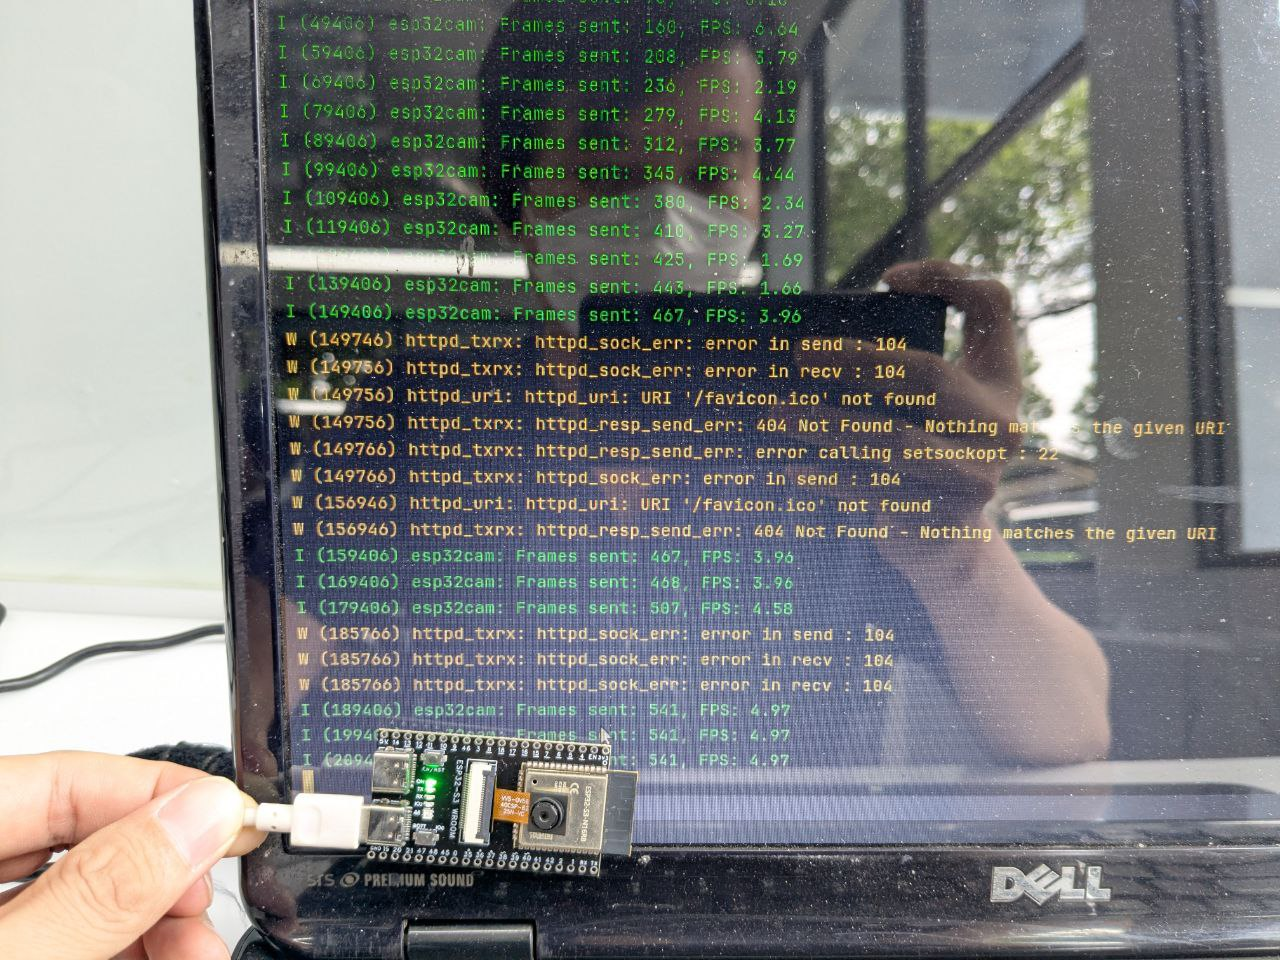
\includegraphics[width=0.8\textwidth]{figures/module2_real_log.jpg}
    \caption{Dashboard hiển thị bản tin MQTT từ thiết bị ESP32.}
    \label{fig:module2_real_log}
\end{figure}

\textit{Kết luận:} Hệ thống phát hiện và xử lý cảnh báo té ngã thành công, kích hoạt đồng thời nhiều kênh cảnh báo.

\subsection{Module Camera và truyền hình ảnh}
Mô-đun ESP32-CAM được kiểm tra để xác nhận khả năng kết nối Wi-Fi và phát luồng hình ảnh qua HTTP.  
Kết quả log cho thấy camera được nhận diện đúng (OV5640), server HTTP đã khởi động và tốc độ khung hình trung bình dao động trong khoảng 3.5–5 FPS.

\begin{minted}[fontsize=\footnotesize,breaklines]{text}
I (8936) esp32cam: Got IP: 10.110.87.85
I (9266) camera: Detected OV5640 camera
I (10006) esp32cam: HTTP server started
I (20006) esp32cam: Frames sent: 50, FPS: 5.87
I (40006) esp32cam: Frames sent: 146, FPS: 4.46
\end{minted}

\begin{figure}[H]
    \centering
    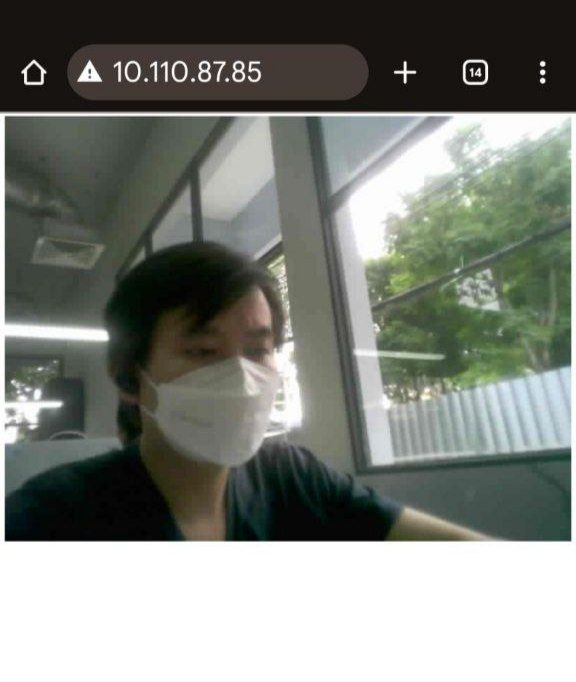
\includegraphics[width=0.8\textwidth]{figures/module1_stream_example.jpg}
    \caption{Luồng hình ảnh phát từ mô-đun ESP32-CAM qua HTTP.}
    \label{fig:camera_stream}
\end{figure}

\textit{Kết luận:} Mô-đun camera hoạt động ổn định, cho phép giám sát hình ảnh trực tiếp phục vụ xác minh sự kiện té ngã.

\subsection{Đánh giá thực nghiệm cảm biến và dữ liệu thu thập}
\subsubsection*{Quy trình thử nghiệm}
Để đánh giá hiệu quả hoạt động của hệ thống trong thực tế, quy trình thử nghiệm được tiến hành theo các bước:
\begin{enumerate}
    \item Nạp chương trình vào ESP32 bằng \texttt{idf.py flash monitor}.  
    \item Giả lập tình huống té ngã bằng cách lắc mạnh hoặc thả nhẹ thiết bị.  
    \item Quan sát log hệ thống để xác nhận sự kiện.  
    \item Kiểm tra tính năng gửi cảnh báo SMS với dữ liệu GPS.  
    \item Lặp lại nhiều lần để đánh giá tính ổn định và độ nhạy.
\end{enumerate}

\subsubsection*{Phân tích dữ liệu cảm biến}
Trong quá trình thử nghiệm, dữ liệu MPU6050 được thu thập cho hai trạng thái: \textbf{té ngã} và \textbf{bình thường}.  
Các bảng dưới đây trình bày toàn bộ dữ liệu đã ghi nhận.

\begin{table}[h]
\centering
\caption{Dữ liệu trong tình huống té ngã}
\label{tab:fall_data}
\begin{tabular}{|c|c|c|c|c|c|c|c|}
\hline
\textbf{Gyro X} & \textbf{Gyro Y} & \textbf{Gyro Z} & \textbf{Gyro Mag} & \textbf{Accel X} & \textbf{Accel Y} & \textbf{Accel Z} & \textbf{Accel Mag} \\
\hline
129.60 & -36.77 & 29.19 & 137.84 & 0.65 & 0.79 & -0.79 & 1.29 \\
-43.90 & 214.79 & 52.97 & 225.54 & 0.53 & 2.00 & -2.00 & 2.88 \\
158.75 & 250.13 & 134.18 & 325.22 & -1.18 & 1.72 & 1.56 & 2.61 \\
-250.14 & -246.07 & -250.14 & 430.91 & 1.11 & 2.00 & -2.00 & 3.04 \\
242.56 & 250.13 & 250.13 & 428.91 & -1.33 & -2.00 & 2.00 & 3.13 \\
-11.60 & -146.43 & -169.58 & 224.35 & 1.80 & 2.00 & -2.00 & 3.35 \\
201.32 & 238.97 & 250.13 & 400.25 & -2.00 & 0.21 & 2.00 & 2.84 \\
-250.14 & -250.14 & -250.14 & 433.25 & 0.55 & 0.23 & -0.37 & 0.69 \\
\hline
\end{tabular}
\end{table}

\begin{table}[h]
\centering
\caption{Dữ liệu trong tình huống bình thường}
\label{tab:normal_data}
\begin{tabular}{|c|c|c|c|c|c|c|c|}
\hline
\textbf{Gyro X} & \textbf{Gyro Y} & \textbf{Gyro Z} & \textbf{Gyro Mag} & \textbf{Accel X} & \textbf{Accel Y} & \textbf{Accel Z} & \textbf{Accel Mag} \\
\hline
1.27 & -1.46 & 0.51 & 2.00 & -0.03 & 0.01 & -0.96 & 0.96 \\
1.07 & -0.95 & 0.53 & 1.52 & -0.04 & 0.02 & -0.97 & 0.97 \\
1.18 & -1.36 & 0.73 & 1.94 & -0.03 & 0.02 & -0.97 & 0.97 \\
1.03 & -1.02 & 0.40 & 1.50 & -0.03 & 0.01 & -0.97 & 0.97 \\
1.37 & -1.08 & 0.58 & 1.84 & -0.03 & 0.01 & -0.97 & 0.97 \\
0.77 & -0.83 & 0.47 & 1.23 & -0.03 & 0.01 & -0.97 & 0.97 \\
1.02 & -0.37 & 0.77 & 1.33 & -0.03 & 0.01 & -0.97 & 0.97 \\
\hline
\end{tabular}
\end{table}

Ngoài ra, dữ liệu GPS thu được từ mô-đun 4G/GPS trong các lần thử nghiệm ngoài trời cũng được ghi lại:

\begin{table}[h]
\centering
\caption{Dữ liệu GPS thu được từ mô-đun 4G/GPS}
\label{tab:gps_data}
\begin{tabular}{|c|c|c|c|c|c|c|}
\hline
\textbf{Time (UTC)} & \textbf{Latitude} & \textbf{Longitude} & \textbf{Altitude (m)} & \textbf{Fix Mode} & \textbf{Date} & \textbf{Satellites} \\
\hline
132517.00 & 1053.3115N & 10646.7839E & 5.07 & 3 & 240425 & 07 \\
132517.00 & 1053.3115N & 10646.7839E & 5.07 & 3 & 240425 & 07 \\
132540.00 & 1053.3117N & 10646.7840E & 5.05 & 3 & 240425 & 07 \\
132540.00 & 1053.3117N & 10646.7840E & 5.05 & 3 & 240425 & 07 \\
132627.00 & 1053.3107N & 10646.7839E & 5.02 & 3 & 240425 & 07 \\
132627.00 & 1053.3107N & 10646.7839E & 5.02 & 3 & 240425 & 07 \\
\hline
\end{tabular}
\end{table}

\subsubsection*{So sánh dữ liệu}
Để đánh giá sự khác biệt rõ rệt giữa hai trạng thái, dữ liệu được tổng hợp thành các giá trị trung bình:

\begin{table}[h]
\centering
\caption{So sánh dữ liệu té ngã và bình thường}
\label{tab:comparison}
\begin{tabular}{|l|c|c|}
\hline
\textbf{Thông số} & \textbf{Trung bình té ngã} & \textbf{Trung bình bình thường} \\
\hline
Gyro X (deg/s) & 22.06 & 1.10 \\
Gyro Y (deg/s) & 34.33 & -1.03 \\
Gyro Z (deg/s) & 5.84  & 0.57 \\
Gyro Mag (deg/s) & 325.78 & 1.63 \\
Accel X (g)   & 0.02  & -0.03 \\
Accel Y (g)   & 0.87  & 0.01 \\
Accel Z (g)   & -0.20 & -0.97 \\
Accel Mag (g) & 2.48  & 0.97 \\
\hline
\end{tabular}
\end{table}

\textit{Kết luận:} Dữ liệu cảm biến cho thấy sự khác biệt rõ rệt giữa hai trạng thái. Đặc biệt, \textbf{Accel Mag} và \textbf{Gyro Mag} là chỉ báo hiệu quả để phát hiện té ngã, cung cấp cơ sở thực nghiệm cho việc tinh chỉnh ngưỡng phát hiện và giảm thiểu cảnh báo sai.

\subsection{Mô-đun nhận diện hình ảnh (Python)}
\label{sec:python_vision}

Mô-đun nhận diện hình ảnh được xây dựng bằng Python nhằm thực hiện các chức năng: thu nhận luồng dữ liệu từ camera, triển khai mô hình học sâu để dựng khung xương (skeleton), đồng thời tích hợp với hệ thống gửi cảnh báo qua MQTT và Telegram. Ngoài ra, mô-đun còn ghi log vào cơ sở dữ liệu SQLite và duy trì kết nối với Asterisk Management Interface (AMI).  

Trong quá trình thử nghiệm, hệ thống được khởi động trực tiếp từ môi trường ảo Python. Các tiến trình chính được khởi tạo bao gồm: \texttt{mqtt\_listener}, \texttt{mqtt\_processor}, \texttt{camera\_processing} và \texttt{heartbeat}. Log tiêu biểu minh họa kết quả thử nghiệm được trình bày dưới đây.

Dưới đây là hình ảnh \ref{fig:python_runing_log}thực tế Python xử lý ảnh và điều phối các tác vụ log ra monitor
\begin{figure}[H]
    \centering
    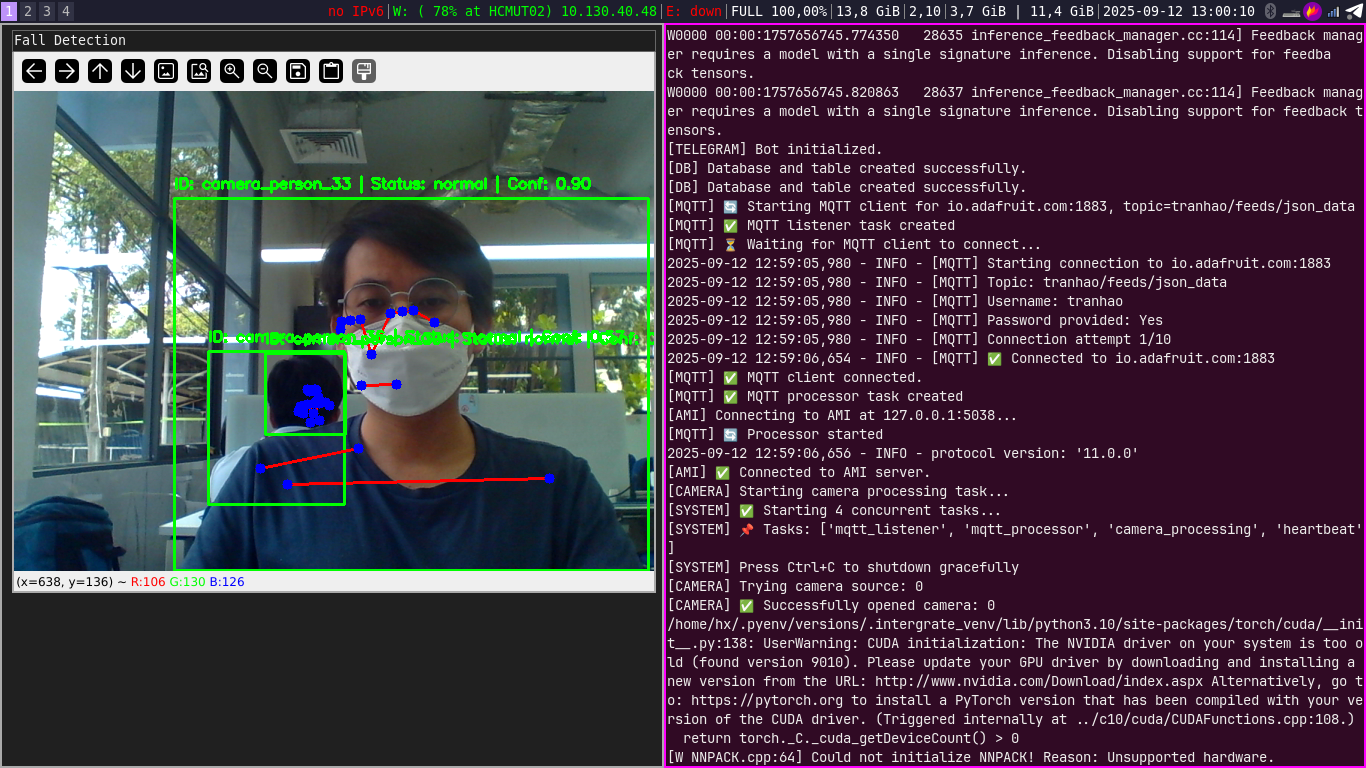
\includegraphics[width=0.8\textwidth]{figures/python_runing_log.png}
    \caption{Dashboard hiển thị bản tin MQTT từ thiết bị ESP32.}
    \label{fig:python_runing_log}
\end{figure}

\subsubsection*{Log thực nghiệm}
\begin{minted}[fontsize=\footnotesize,breaklines]{text}
[SYSTEM] 🚀 Starting Fall Detection System...
[SYSTEM] Initializing modules...
INFO: Created TensorFlow Lite XNNPACK delegate for CPU.
[TELEGRAM] Bot initialized.
[DB] Database and table created successfully.
[MQTT] 🔄 Starting MQTT client for io.adafruit.com:1883, topic=tranhao/feeds/json_data
[MQTT] ✅ MQTT client connected.
[AMI] ✅ Connected to AMI server.
[CAMERA] Starting camera processing task...
[SYSTEM] ✅ Starting 4 concurrent tasks...
[CAMERA] ✅ Successfully opened camera: 0
/home/hx/.pyenv/versions/.intergrate_venv/lib/python3.10/site-packages/torch/cuda/__init__.py:138:
UserWarning: CUDA initialization: The NVIDIA driver on your system is too old (found version 9010)...
\end{minted}

\subsubsection*{Phân tích kết quả}
Từ log trên có thể rút ra các nhận xét sau:
\begin{itemize}
    \item \textbf{Khởi tạo hệ thống:} Các mô-đun cốt lõi (MQTT, cơ sở dữ liệu, Telegram bot, AMI) đều được khởi tạo thành công. Điều này chứng minh khả năng tích hợp của hệ thống Python với hạ tầng dịch vụ bên ngoài.
    \item \textbf{Xử lý camera:} Camera nội bộ được mở thành công (\texttt{Successfully opened camera: 0}), khẳng định rằng mô-đun xử lý hình ảnh đã sẵn sàng cho tác vụ nhận diện skeleton.
    \item \textbf{Mô hình học máy:} TensorFlow Lite XNNPACK delegate cho CPU được khởi động thành công. Cảnh báo từ thư viện CUDA cho thấy driver GPU không tương thích, tuy nhiên hệ thống vẫn hoạt động bình thường trên nền tảng CPU.
    \item \textbf{Đa nhiệm đồng thời:} Bốn tác vụ chính (\texttt{mqtt\_listener}, \texttt{mqtt\_processor}, \texttt{camera\_processing}, \texttt{heartbeat}) được khởi chạy song song, thể hiện tính ổn định của pipeline xử lý.
\end{itemize}

\subsubsection*{} 
Kết quả thử nghiệm chứng minh rằng mô-đun Python đã hoạt động đúng chức năng, bảo đảm khả năng thu nhận dữ liệu camera, chạy nhận diện hình ảnh, đồng bộ dữ liệu qua MQTT, và kích hoạt các kênh cảnh báo. Hệ thống tuy có hạn chế về hỗ trợ CUDA (do phiên bản driver cũ) nhưng không ảnh hưởng đến quá trình thực thi trên CPU. Đây là minh chứng cho tính ổn định và khả năng triển khai của giải pháp trong điều kiện phần cứng phổ thông.

\subsection{Kênh cảnh báo Telegram}
\label{sec:telegram_alert}

Hệ thống Telegram Bot đóng vai trò là kênh cảnh báo trực quan, giúp gửi thông báo đến người dùng ngay khi phát hiện té ngã.  
Cơ chế hoạt động được chia thành hai hướng:
\begin{itemize}
    \item \textbf{Từ mô-đun phần cứng (ESP32 + 4G/GPS):} Khi xảy ra sự kiện té ngã, bản tin MQTT hoặc SMS được phát ra từ thiết bị. Hệ thống trung tâm sau đó chuyển tiếp nội dung này đến người dùng thông qua Telegram.
    \item \textbf{Từ mô-đun xử lý hình ảnh (Python):} Khi nhận diện được té ngã qua camera và skeleton, hệ thống Python trực tiếp gửi cảnh báo đến Telegram, kèm thông tin chi tiết.
\end{itemize}

\subsubsection*{Log minh họa}
\begin{minted}[fontsize=\footnotesize,breaklines]{text}
[TELEGRAM] Bot initialized.
2025-09-12 12:55:17,594 - INFO - HTTP Request: POST
https://api.telegram.org/botXXXX/sendMessage "HTTP/1.1 200 OK"
[TELEGRAM] Test message sent successfully.
I (159151) SIM4G_GPS: SMS request queued successfully
I (159191) SIM4G_GPS: MQTT alert published successfully.
I (159881) SIM4G_AT: SMS sent successfully.
\end{minted}

\subsubsection*{Kết quả thử nghiệm}
Trong quá trình chạy thử, Telegram Bot đã nhận thành công cảnh báo từ cả hai nguồn:
\begin{itemize}
    \item \textbf{Mô-đun phần cứng:} gửi cảnh báo khi hệ thống ESP32 phát hiện té ngã và kích hoạt chuỗi xử lý SMS/MQTT.
    \item \textbf{Mô-đun Python:} gửi cảnh báo trực tiếp khi nhận diện té ngã qua camera và skeleton tracking.
\end{itemize}

\begin{figure}[H]
    \centering
    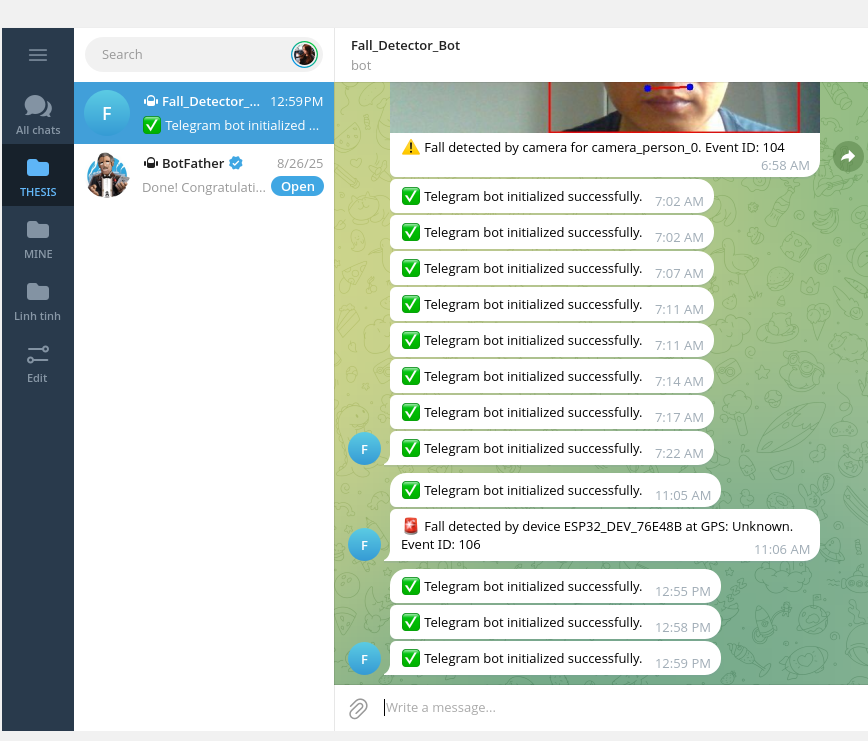
\includegraphics[width=0.8\textwidth]{figures/telegram_fall_module1_send.png}
    \caption{Thông báo cảnh báo té ngã từ mô-đun phần cứng (ESP32) qua Telegram.}
    \label{fig:telegram_hw}
\end{figure}

\begin{figure}[H]
    \centering
    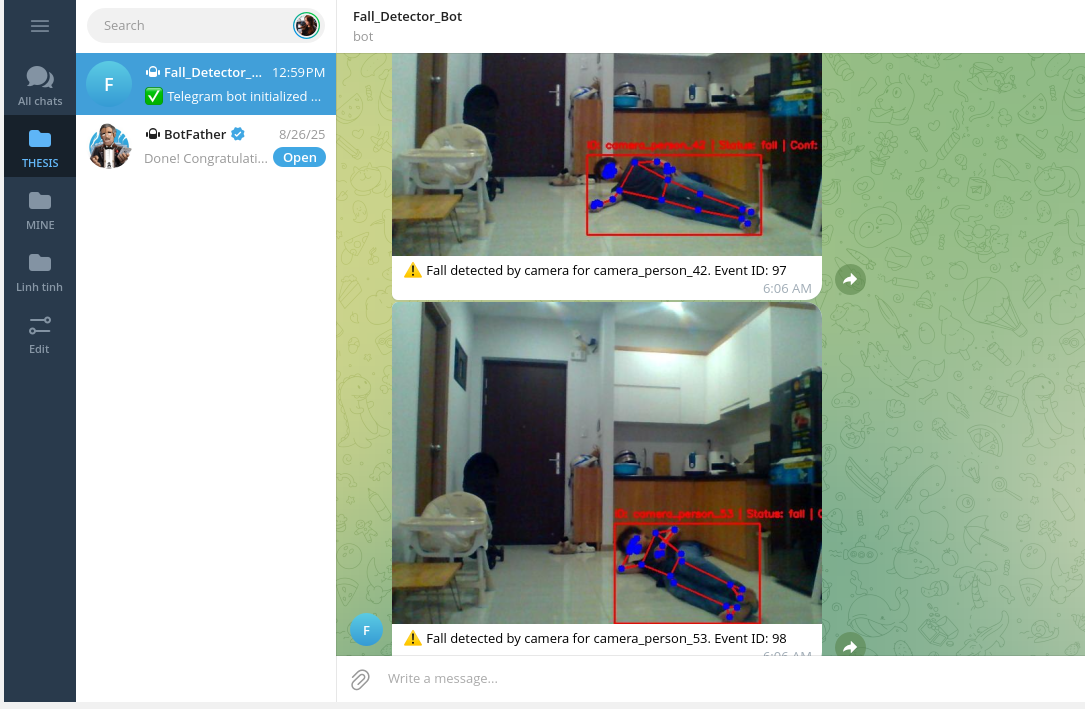
\includegraphics[width=0.8\textwidth]{figures/telegram_python_fall_send.png}
    \caption{Thông báo cảnh báo té ngã từ mô-đun xử lý hình ảnh Python qua Telegram.}
    \label{fig:telegram_python}
\end{figure}

\subsubsection*{Nhận xét}
Kết quả chứng minh rằng Telegram Bot đã hoạt động ổn định, đóng vai trò là cầu nối quan trọng giữa hệ thống phát hiện té ngã và người dùng cuối.  
Việc kết hợp cả hai nguồn cảnh báo (thiết bị phần cứng và mô-đun xử lý hình ảnh) giúp tăng độ tin cậy và giảm thiểu khả năng bỏ sót sự kiện.
\paragraph{}  
Các thử nghiệm chức năng trên khẳng định rằng từng thành phần của hệ thống đã hoạt động đúng theo hướng mong muốn.
